\chapter{Implementation}

%The implementation should discuss any issues you encountered as you tried to implement your design. During the work, you might have found that elements of your design were unnecessary or overly complex; perhaps third-party libraries were available that simplified some of the functions that you intended to implement. If things were easier in some areas, then how did you adapt your project to take account of your findings?
%
%It is more likely that things were more complex than you first thought. In particular, were there any problems or difficulties that you found during implementation that you had to address? Did such problems simply delay you or were they more significant?
%
%You can conclude this section by reviewing the end of the implementation stage against the planned requirements. 

\section{Code Implementation \& Third-Party libraries}
As seen below the Website and Discord bot have been split up into two separate sections because during implementation to help keep the systems separate. This helps with code maintainability, readability and allows the administrator who sets up this project to deploy the website and bot services on different containers or networks. For more information of third party libraries please see appendix A.

\section{Website Building and Final Design}
To create and run the website a set of libraries and Linux packages are used to perform certain tasks. Firstly, the Linux package Apache2 \cite{apache2} is used as the web hosting framework got the website along with the library libapache2-mod-auth-openidc to reroute all incoming traffic to OpenID Connect \cite{OpenID} for user authentication. On top of these the linux tool certbot \cite{certbot} is used to create a Let's Encrypt certificate for the website to enable HTTPS. 

As discussed previously in this document in section \ref{sec1:Research} there were many libraries that were considered when deciding on the website framework. Django \cite{Django} was the framework of choice and it is open-source and free to use on personal projects. It is also very useful as it generates the majority of the code required to create and run a website so most of the code used will be picked up by the system for UAP. Apart from the generated template, a "Django Application" called login that contains the files and code which is used to run the website. I can confirm that the folder, login, is all my own code and should not fall under UAP.

The website pages also use a third party library called bootstrap \cite{bootstrap} that is used to generate responsive mobile-first CSS for the website. The final design of the website ended up being very similar to that of the mockups made in section \ref{sec2:ui} and included below are some images from the final website.

\textbf{Note}: The navigation bars in the images below are smaller than the mockups due to the change in screen size. These images were taken on a 27inch monitor whereas the mockups were made for a 15inch monitor.

\begin{figure}[H]
	\centering
	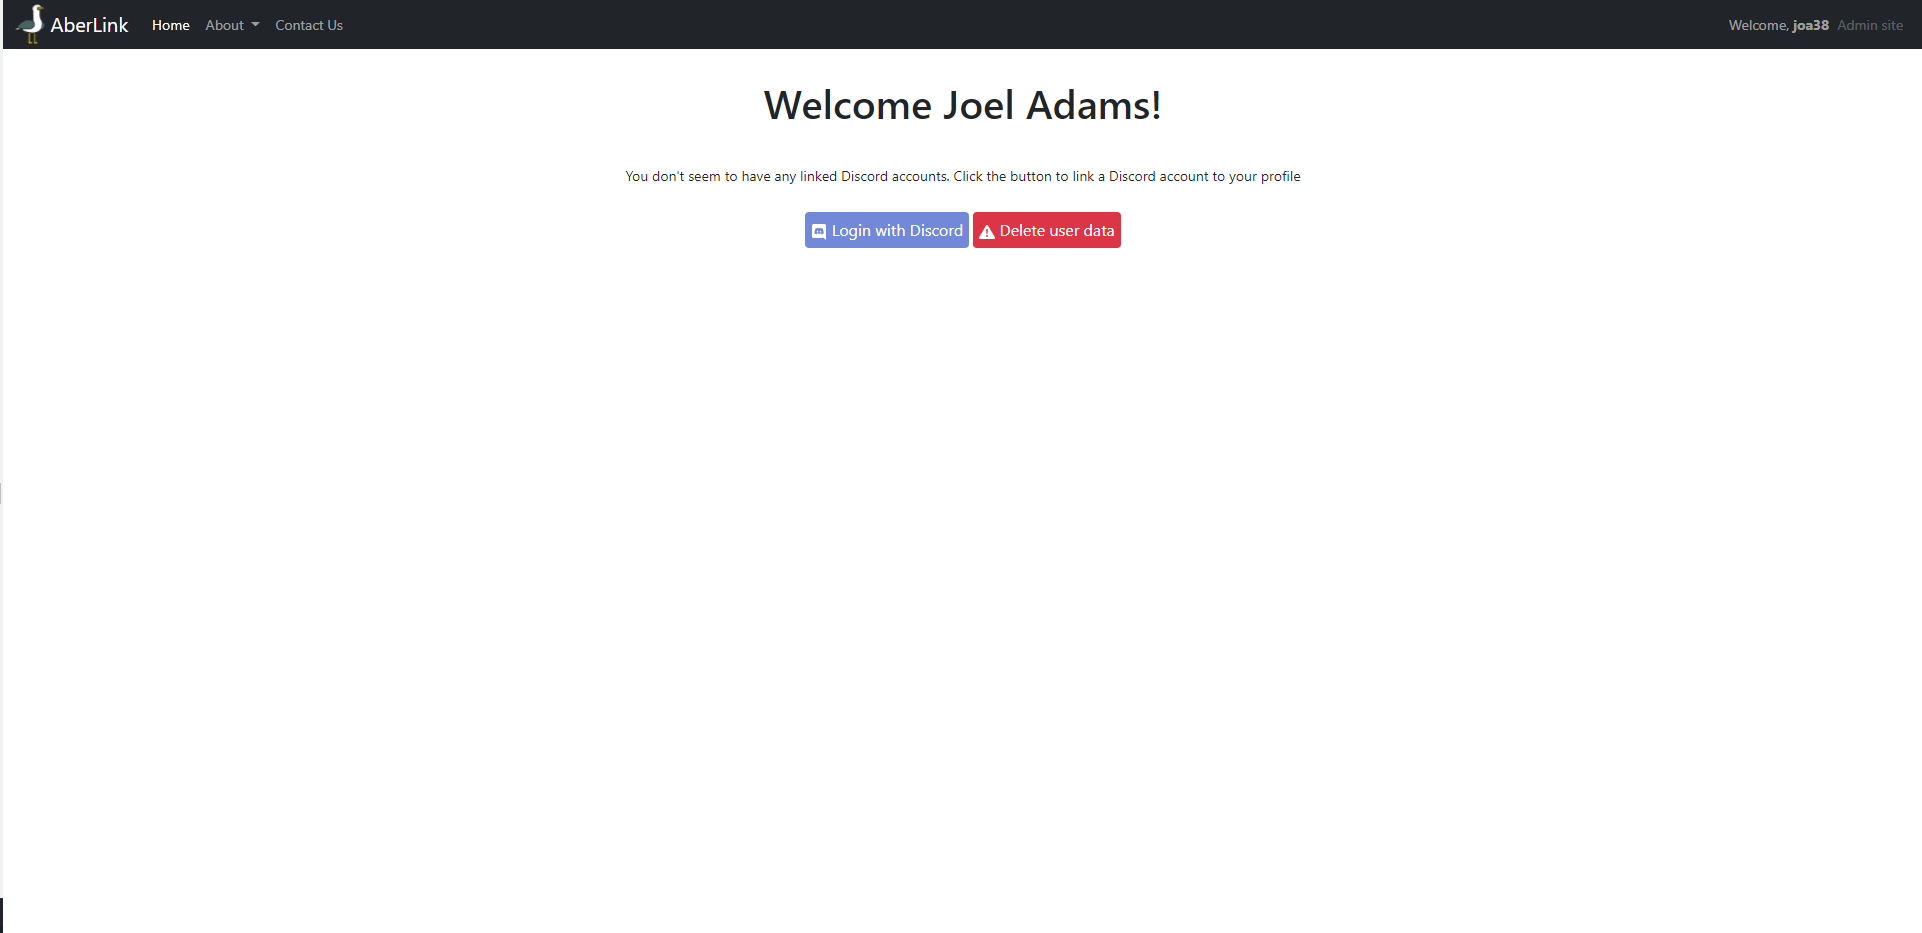
\includegraphics[width=1\linewidth]{Figures/website-acc-0.png}
	\caption{Final website with 0 linked Discord accounts \\\centering\href{https://mmp-joa38.dcs.aber.ac.uk}{https://mmp-joa38.dcs.aber.ac.uk}}
	\label{fig:final-web-acc-0}
\end{figure}

\begin{figure}[H]
	\centering
	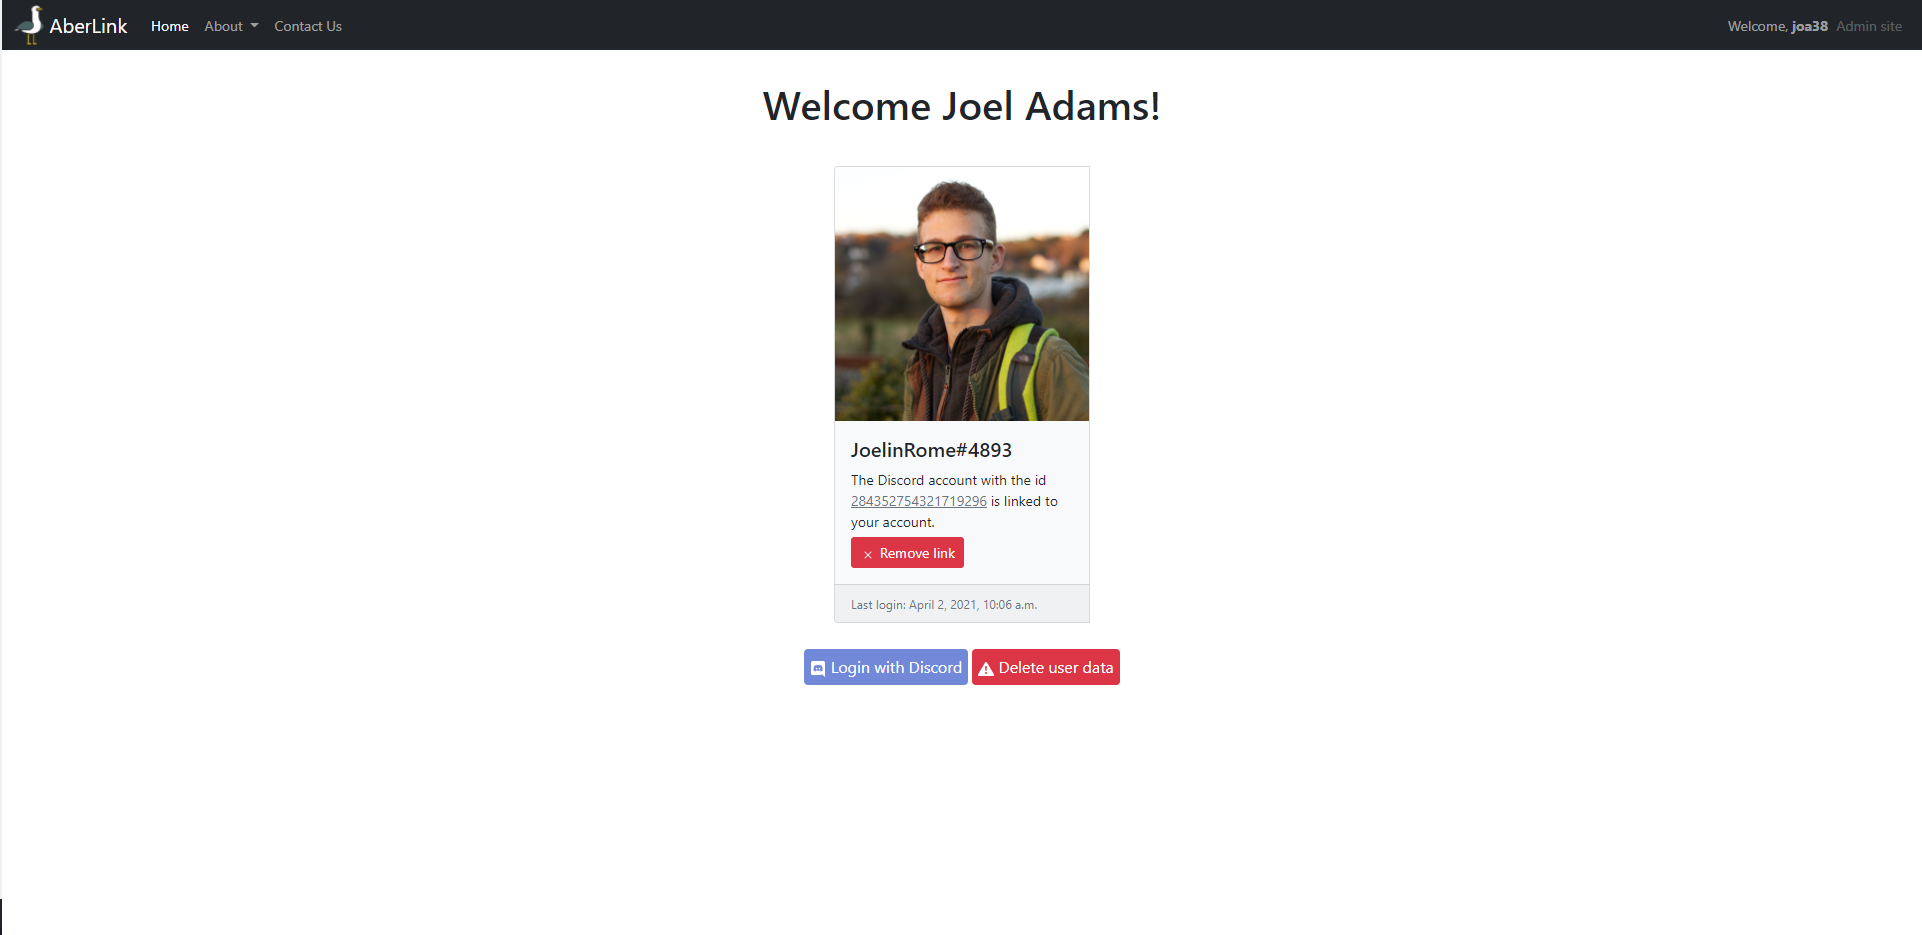
\includegraphics[width=1\linewidth]{Figures/website-acc-1.png}
	\caption{Final website with 1 linked Discord accounts \\\centering\href{https://mmp-joa38.dcs.aber.ac.uk}{https://mmp-joa38.dcs.aber.ac.uk}}
	\label{fig:final-web-acc-1}
\end{figure}

\begin{figure}[H]
	\centering
	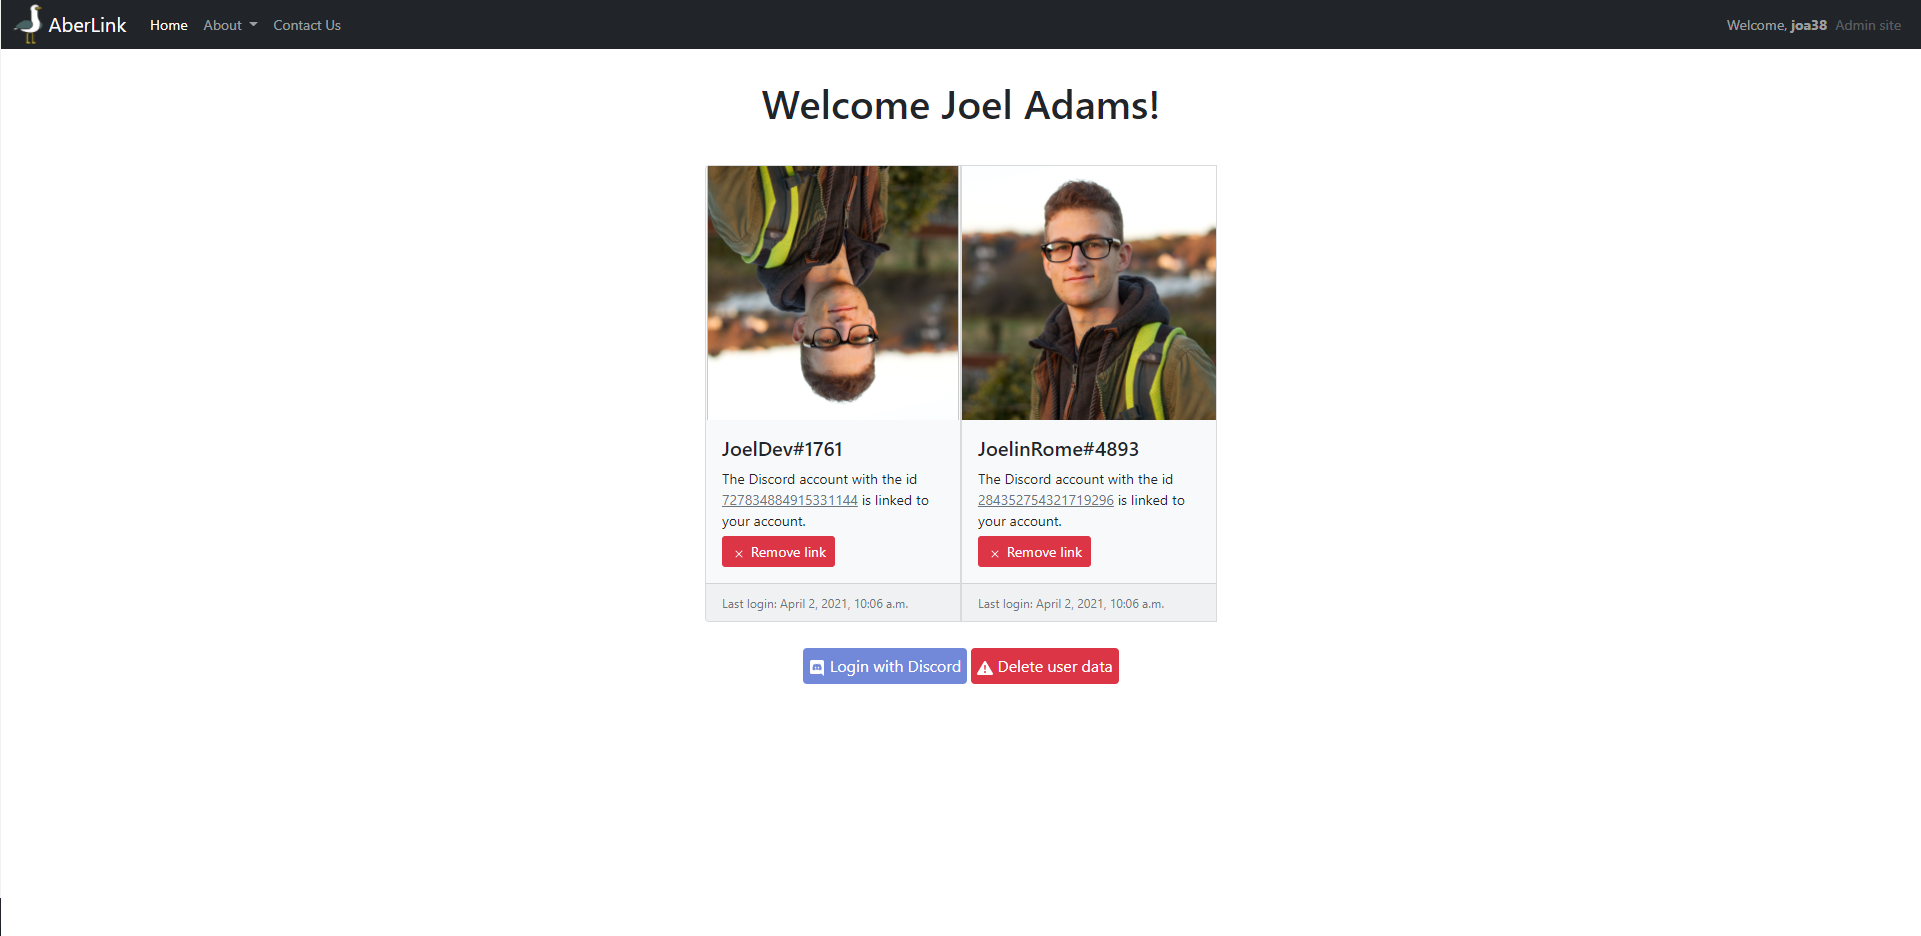
\includegraphics[width=1\linewidth]{Figures/website-acc-2.png}
	\caption{Final website with 2 linked Discord accounts \\\centering\href{https://mmp-joa38.dcs.aber.ac.uk}{https://mmp-joa38.dcs.aber.ac.uk}}
	\label{fig:final-web-acc-2}
\end{figure}

\begin{figure}[H]
	\centering
	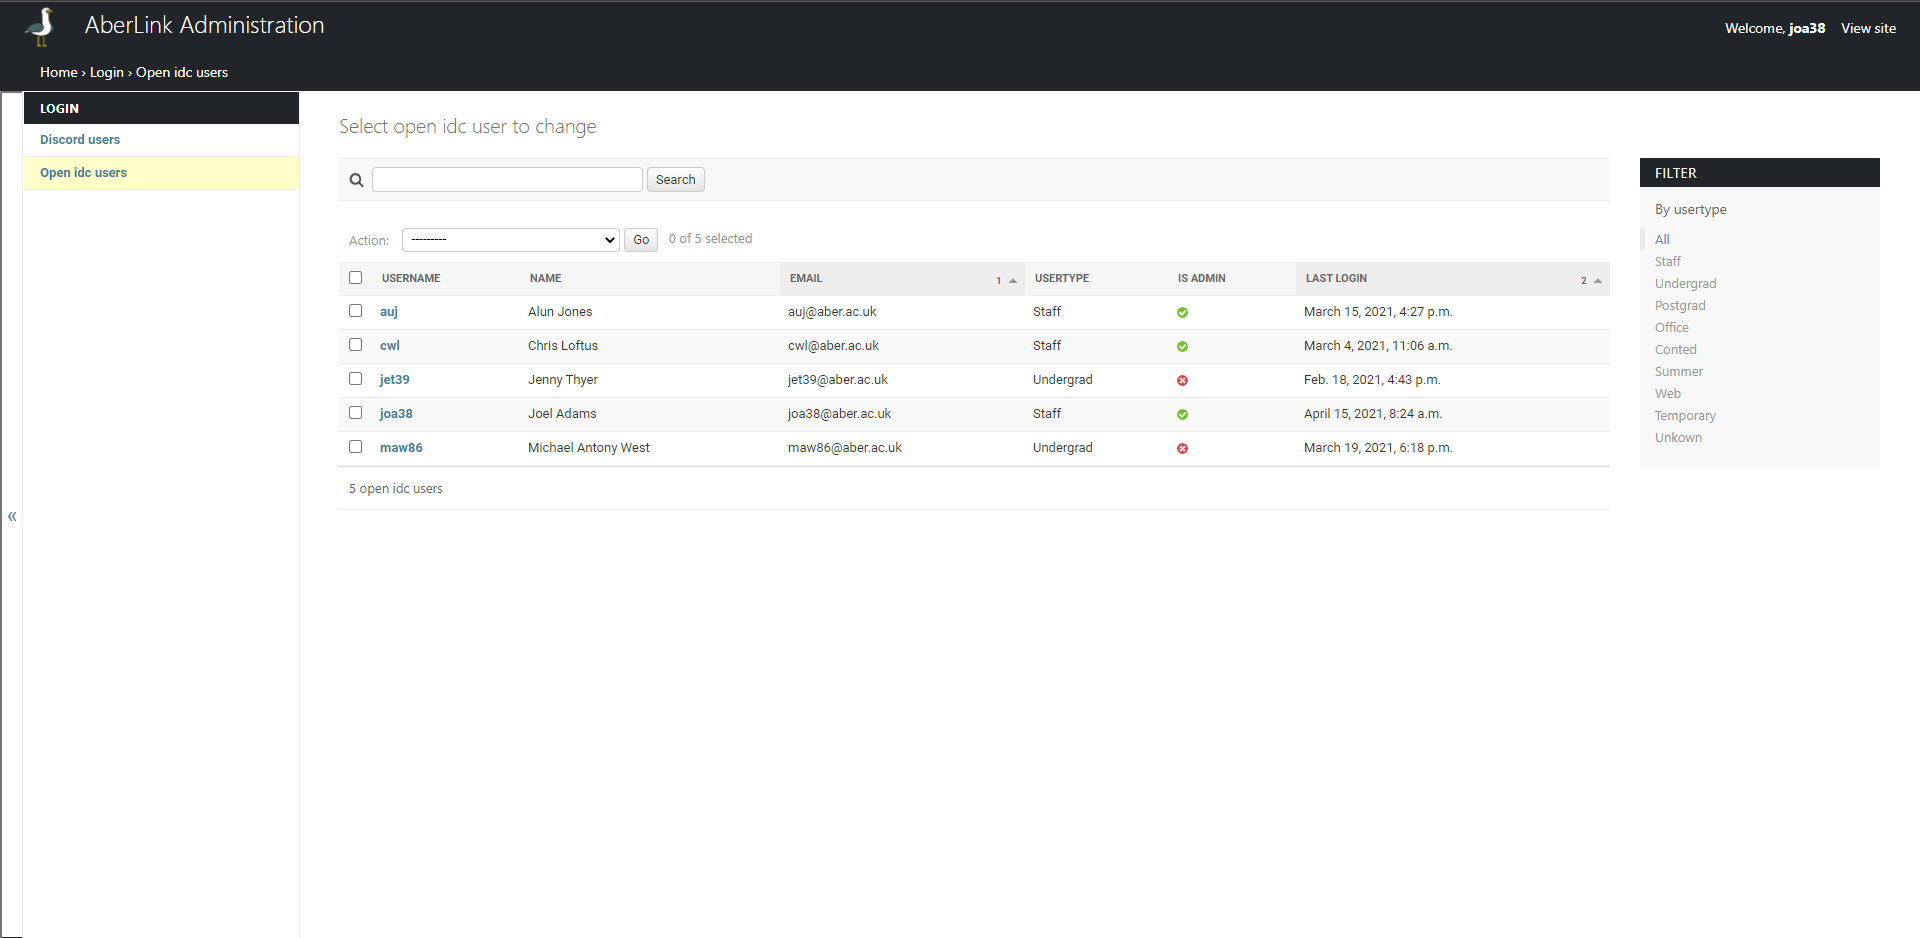
\includegraphics[width=1\linewidth]{Figures/website-admin-openidc.png}
	\caption{Final website Admin page for Aber accounts \\\centering\href{https://mmp-joa38.dcs.aber.ac.uk/admin/login/openidcuser/}{https://mmp-joa38.dcs.aber.ac.uk/admin/login/openidcuser/}}
	\label{fig:final-web-admin-openidc}
\end{figure}

\begin{figure}[H]
	\centering
	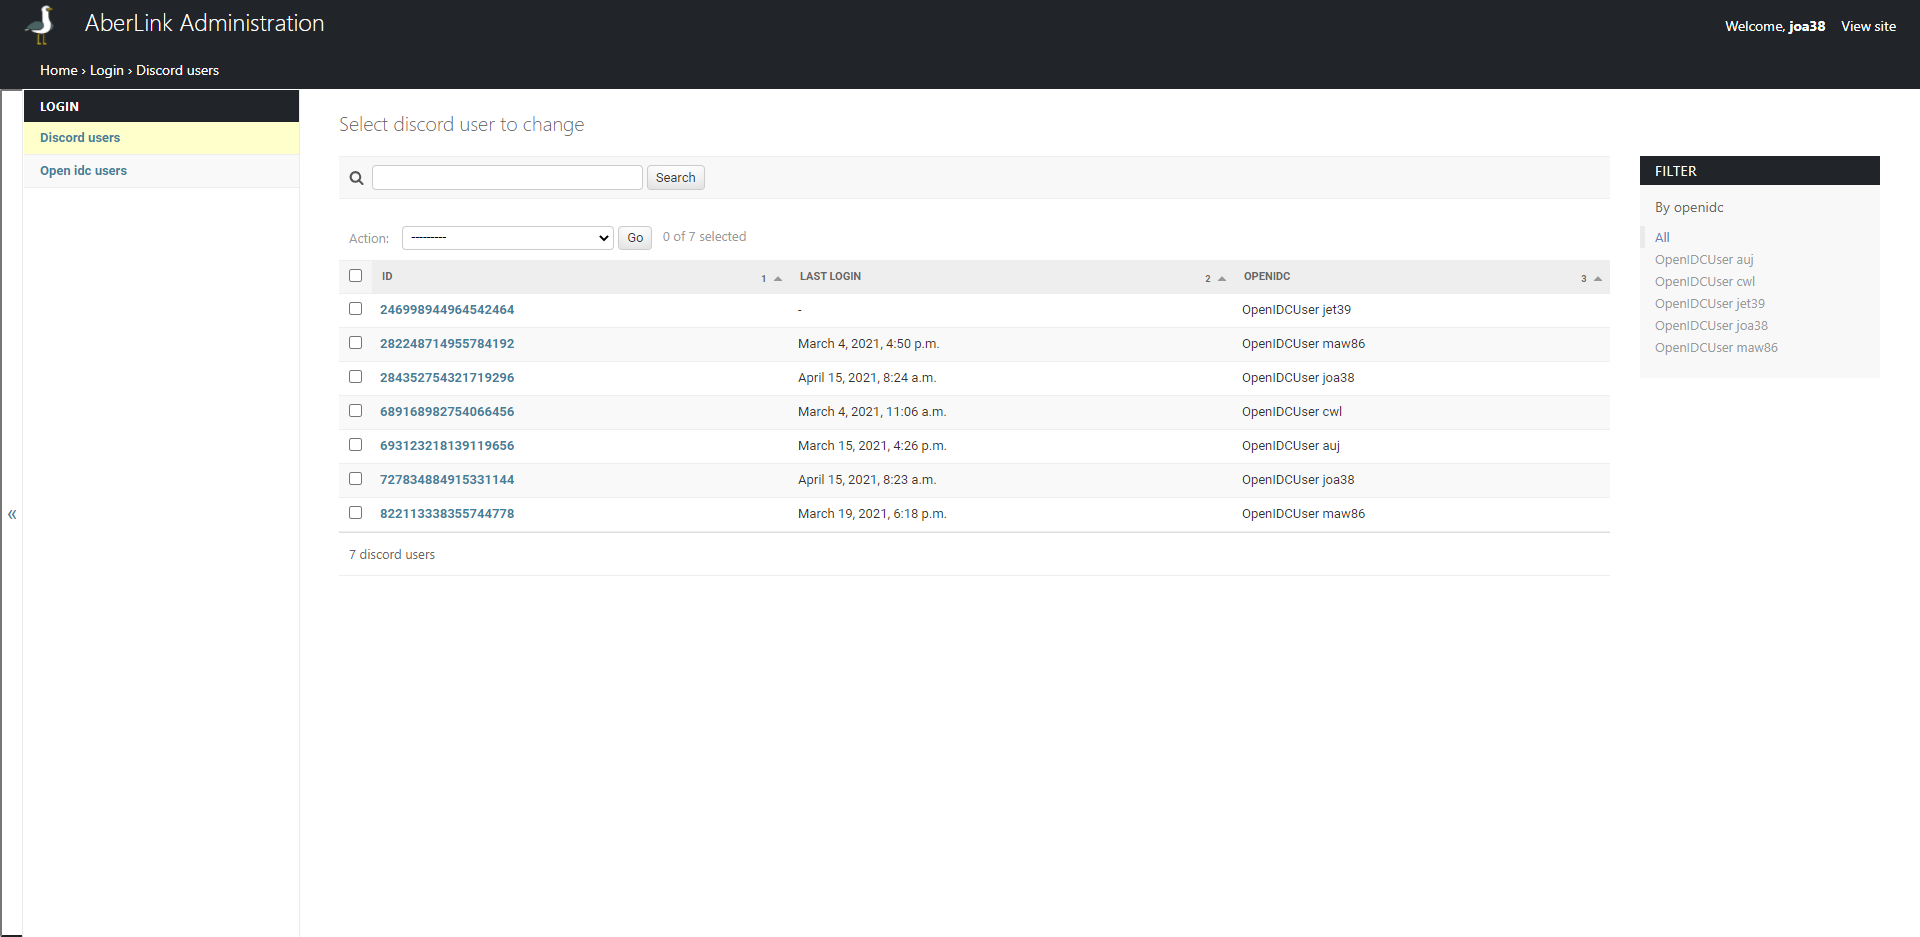
\includegraphics[width=1\linewidth]{Figures/website-admin-discord.png}
	\caption{Final website Admin page for Discord accounts \\\centering\href{https://mmp-joa38.dcs.aber.ac.uk/admin/login/discorduser/}{https://mmp-joa38.dcs.aber.ac.uk/admin/login/discorduser/}}
	\label{fig:final-web-admin-dis}
\end{figure}

Most of the users visiting this website will have not have a clue about this project or any of its policies so included below are the other two webpages created for this project. These pages display information about the project and privacy policy respectively.

\begin{figure}[H]
	\centering
	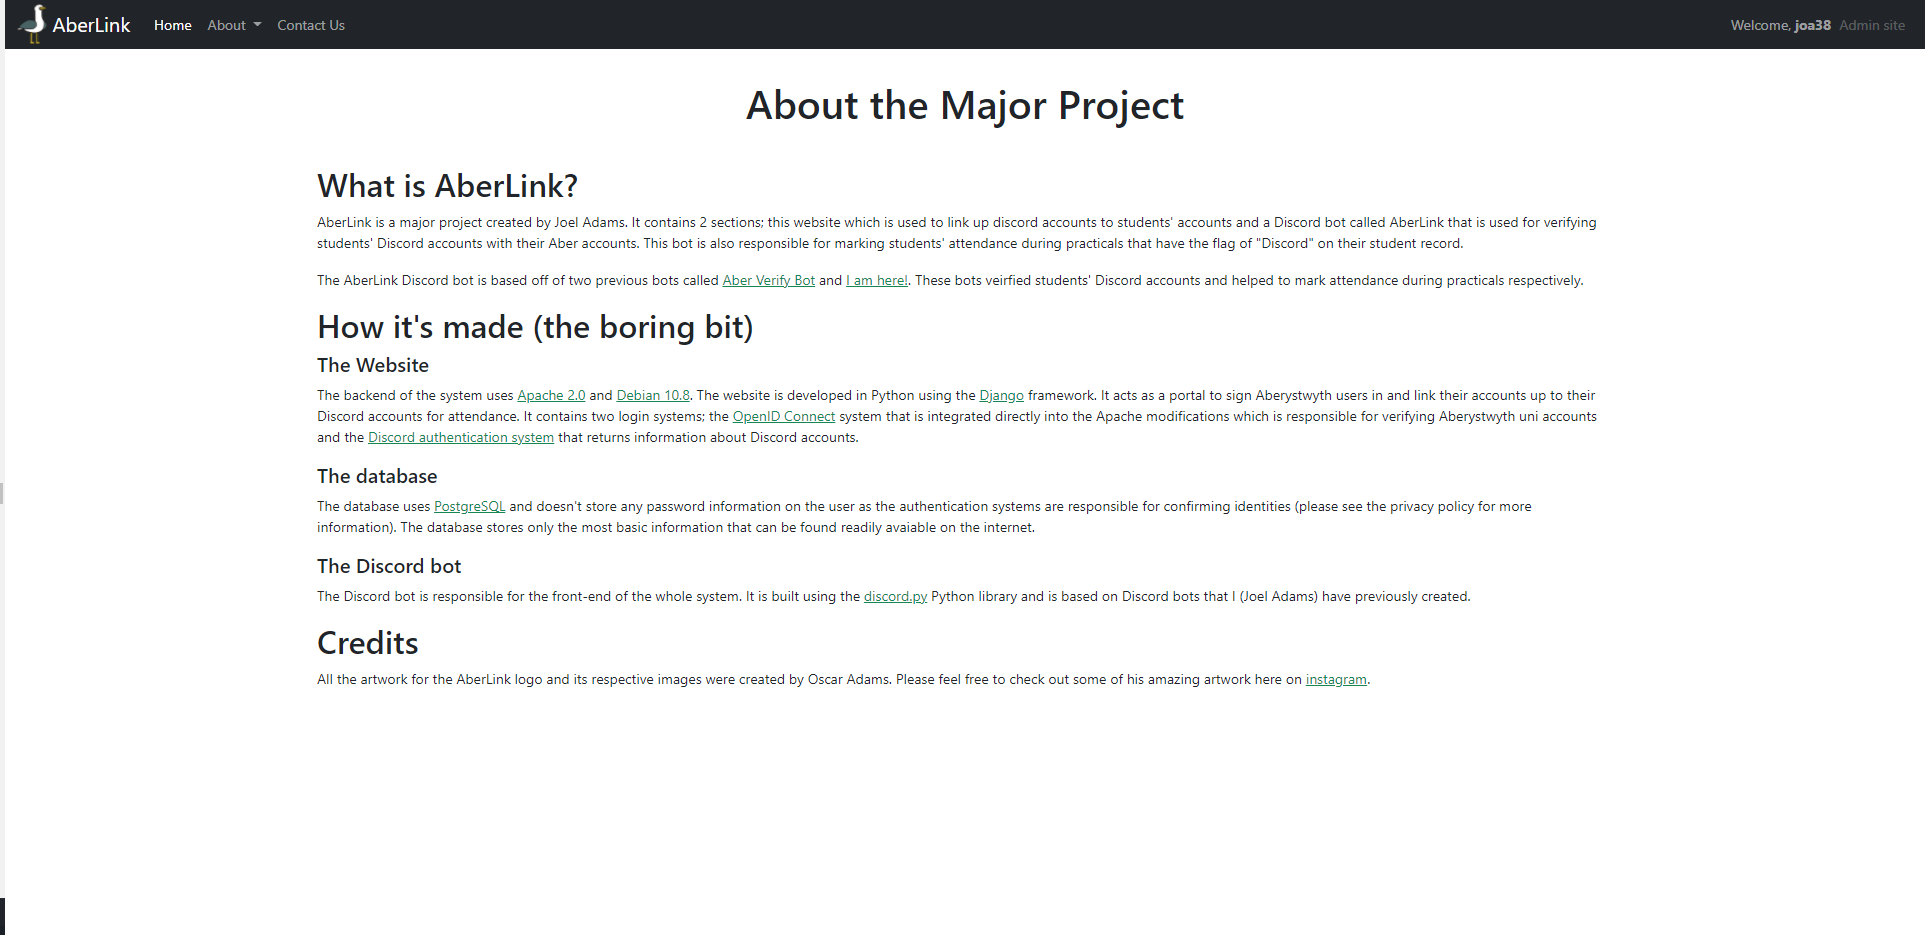
\includegraphics[width=1\linewidth]{Figures/website-mmp.png}
	\caption{Webpage for information on what the project is about \\\centering\href{https://mmp-joa38.dcs.aber.ac.uk/major-project}{https://mmp-joa38.dcs.aber.ac.uk/major-project}}
	\label{fig:final-web-mmp}
\end{figure}

\begin{figure}[H]
	\centering
	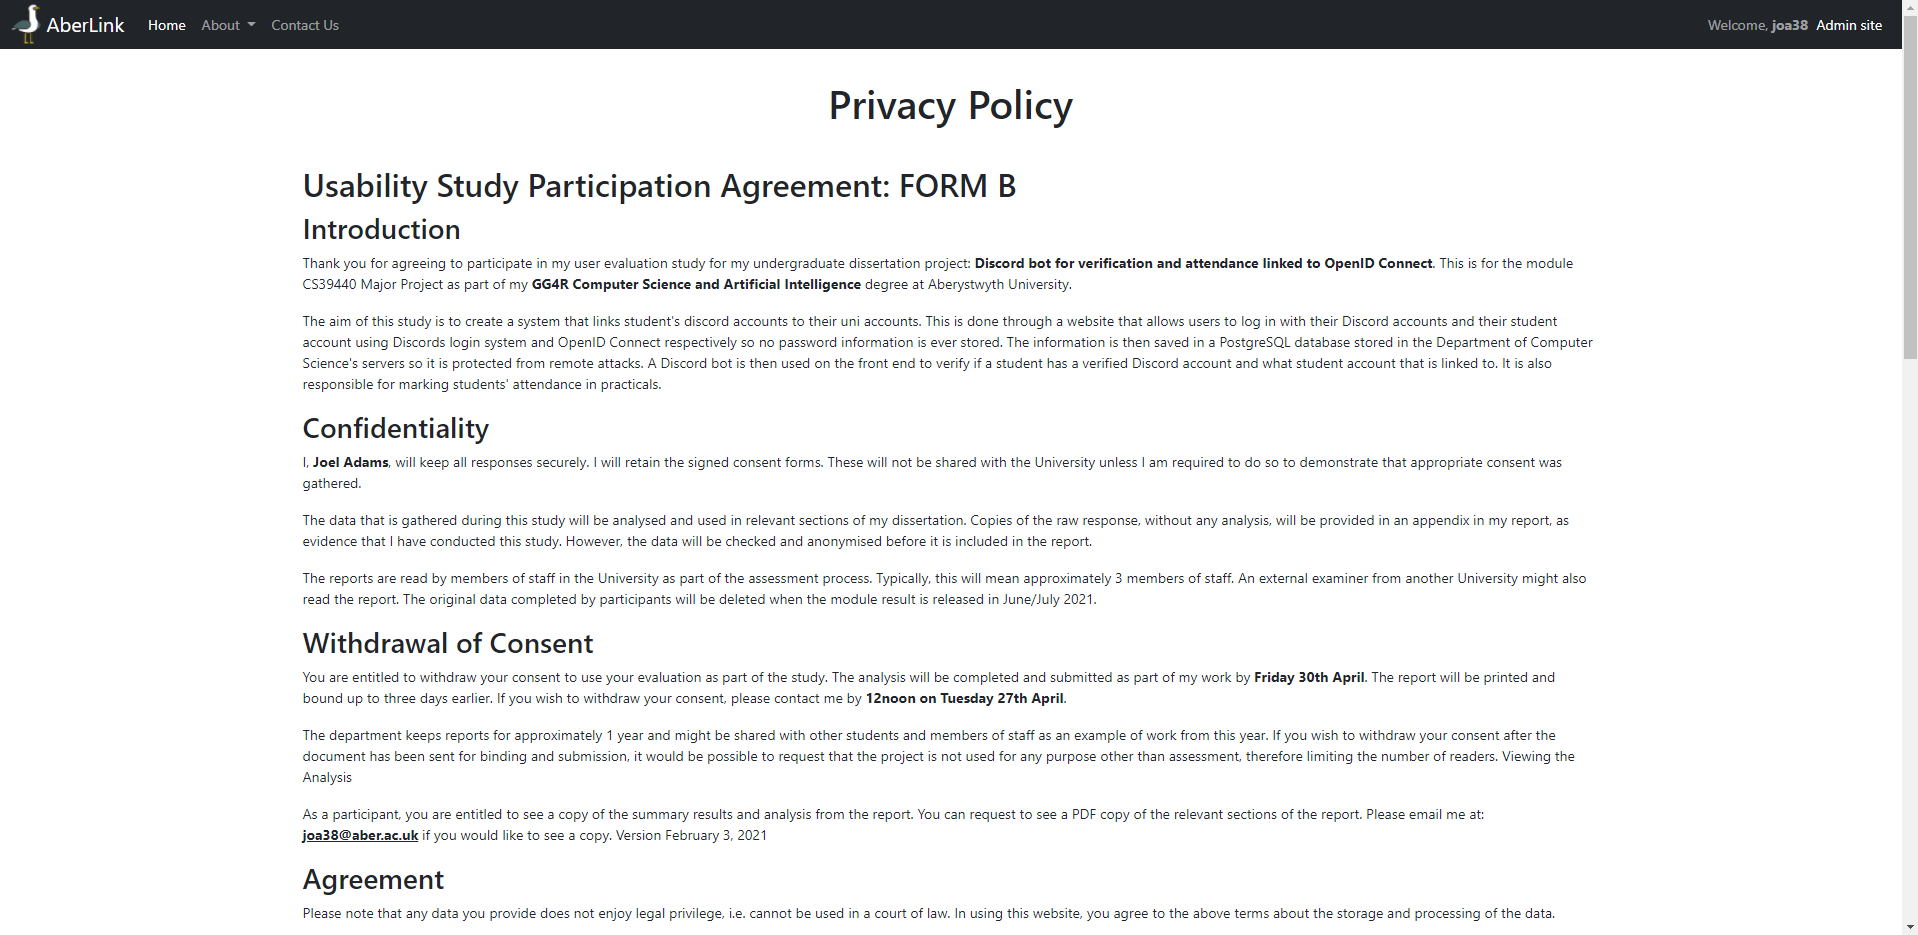
\includegraphics[width=1\linewidth]{Figures/website-privacy-policy.png}
	\caption{Webpage displaying agreement form and Ethics form \\\centering\href{https://mmp-joa38.dcs.aber.ac.uk/privacy-policy}{https://mmp-joa38.dcs.aber.ac.uk/privacy-policy}}
	\label{fig:final-web-privacy-policy}
\end{figure}

\subsection{Complicated Behaviours}

\subsubsection{Retrieving and Displaying Discord Information}
The main complicated behaviour occurs when the user logs into the website and gets redirected to the homepage after they have authenticated one Discord account. When this happens the now logged in Discord account is linked to the OpenID Connect account and their information is saved to the database. As seen in table \ref{tab:dis-table} the only information that gets saved to the database is their Discord ID and time of login, notice how their profile image or name are not saved to the database. This is because this information is subject to change and is not required to be stored in the database. This was done to ensure that the table is normalised to the 3rd normal form. It does however create an issue where the website does not know any information on the connected Discord account account apart from their ID. 

To get around this a function is used that creates an API request to Discord querying information on the connected account. As seen below the function takes in a \verb|QuerySet| that contains a list of connected Discord accounts and then makes an API request to the url \verb|https://discord.com/api/v8/users/{discord_user.id}| with each Discord ID. After it has looped through all the connected accounts it returns an array of JSON objects that contain information on the connected accounts.

\begin{figure}[H]
\begin{lstlisting}[language=Python]
def get_discord_users(discord_users: QuerySet):
"""
uses bot authorisation to get Discord users' info
Returns list of Discord users
"""
json_response = {}
for discord_user in discord_users:
	response = requests.get(f'https://discord.com/api/v8/users/{discord_user.id}', 
	headers={'Authorization': f'Bot {config["DISCORD_TOKEN"]}'
	})
	user = response.json()
	user = {user["id"] : response.json()}
	json_response.update(user)
return json_response
\end{lstlisting}
\caption{Python function to make an API request about connected Discord account}
\label{fig:django-js-json}
\end{figure}

The HTML webpage is then passed this content where it turns the JSON information into a JavaScript function and therefore making it a selectable document element. The document then loops over each Discord account and executes the following JavaScript function to extract information from the JSON object. Once it has extracted the information it replaces the profile picture and name of connected Discord account in the document.

\begin{figure}[H]
\begin{lstlisting}[language=JavaScript]
let json_data = JSON.parse(document.getElementById("discord_user_info").textContent)
let discordAvatar = json_data["{{user.id}}"].avatar
let discordUsername = json_data["{{user.id}}"].username + "#" + json_data["{{user.id}}"].discriminator
document.getElementById("discordAvatar{{forloop.counter}}").src = `https://cdn.discordapp.com/avatars/{{user.id}}/${discordAvatar}.png?size=256`
document.getElementById("discordUsername{{forloop.counter}}").textContent = `${discordUsername}`
\end{lstlisting}
\caption{JavaScript script to extract information from the Discord users JSON object}
\label{fig:django-api-dis}
\end{figure}

\subsubsection{Deleting Account or Unlinking Discord accounts}
This project respects the GDPR regulations and gives users the right to delete their data from the database or unlink a Discord account. This feature was simple to implement but became difficult when I wanted to include popups that would appear when the user tried to delete their account as pictured below. The difficult part about this comes when trying to get information on which account is going to be deleted and ensuring that the correct one is selected.

\begin{figure}[H]
	\centering
	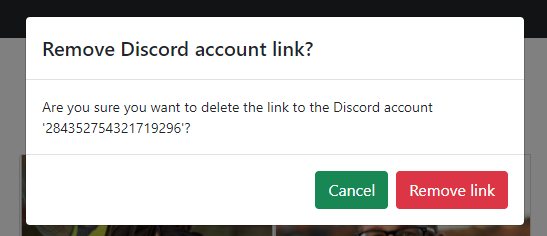
\includegraphics[width=1\textwidth]{Figures/website-discord-modal.png}
	\caption{Example of a popup that appears when a user tried to unlink a Discord account}
	\label{fig:django-modal}
\end{figure}

Implementing this feature was relatively straight forward however getting it to display information on the specific account that would be unlinked was harder than expected. Getting the HTML document to parse information on which button had been pressed in the document was as simple as adding an extra attribute to the button. As seen in the figure below the button contains the attribute \verb|value| that is assigned to the Discord account.

\begin{figure}[H]
\begin{lstlisting}[language=HTML]
<button type="button" id="discordDeleteButton" class="btn btn-danger btn-sm" data-bs-toggle="modal"
	data-bs-target="#discordDeleteButtonModal" value="{{ user.id }}" style="margin-top: 5px;">
\end{lstlisting}
\caption{HTML button to delete a Discord account containing value attribute with the Discord ID}
\label{fig:django-dis-delete-button}
\end{figure}

When the button is pressed it calls a JavaScript script and displays the popup/modal. It then uses the function \verb|event.relatedTarget.getAttribute| to get the information from the button on the account that is linked to it.

\begin{figure}[H]
\begin{lstlisting}[language=JavaScript]
let deleteDiscordAccountModal = document.getElementById('discordDeleteButtonModal')
deleteDiscordAccountModal.addEventListener('show.bs.modal', function (event) {
	// Gets the button and it's data attribute and prints it out in the .modal-body
	let recipient = event.relatedTarget.getAttribute('value')
	deleteDiscordAccountModal.querySelector('.modal-body').textContent = 'Are you sure you want to delete the link to the Discord account \'' + recipient + '\'?'
	document.getElementById('discordIdText').value = recipient
})
\end{lstlisting}
\caption{JavaScript script to get context on the button that has been pressed and edit the popup to include this information}
\label{fig:django-js-modal}
\end{figure}

Once the confirmation button in \ref{fig:django-modal} is pressed the webpage will send a form containing the Discord id via a post request to the same webpage. The Python function for this webpage then detects that a post request has been made and it attempts to find the linked account and remove it from the database.

\begin{figure}[H]
\begin{lstlisting}[language=python]
def openidc_response(request):
	...
	if request.method == 'POST':
	try:
		discord_id = request.POST.get("discord_id")
		DiscordUser.objects.filter(id=discord_id).delete()
	except KeyError:
		pass
	...
\end{lstlisting}
\caption{Extract from Django Python function to display the home page and handle post requests to remove Discord accounts}
\label{fig:django-view-post}
\end{figure}

\section{Discord Bot}
The Discord bots (AberLink) implementation uses many of the design principles discussed in section \ref{sec2:discord} of this document.

\subsection{Setup and Configuration}\label{sec3:discord-setup}
The bot contains a main file called AberLink.py that configures the bot giving it all the required permissions/settings to run. It loads the sensitive credentials from a .env file using the Python library dotenv \cite{dotenv}. This file contains key-value pairs that hold the Discord bot token that is accessible from the Discord developer portal \url{https://discord.com/developers/applications} and information required for the bot to connect to the database.

\begin{figure}[H]
\begin{lstlisting}[language=Python]
# load the private discord token from .env file.
load_dotenv()
TOKEN = os.getenv('DISCORD_TOKEN')
WEBSITE = os.getenv('WEBSITE_URL')

# Initialise the database connection
PostgreSQL.connect()

# Initialise the Bot object with an accessible help Command object
helpCommand = DefaultHelpCommand()

bot = commands.Bot(
    command_prefix="!",
    help_command=helpCommand,
    intents=discord.Intents.all(),
)

bot.run(TOKEN)
\end{lstlisting}
\caption{Snippet of code from AberLink.py main Discord bot file}
\label{fig:discord-main-file}
\end{figure}

As seen in the figure above the key value pair for the \verb|DISCORD_TOKEN| is loaded in from the file and then used at the end of the code extract to run the bot. In the middle we see an important section called \verb|commands.Bot| that configures the bot with key information such as which prefix to use to call commands. E.g. if the prefix is set to \verb|!| then a command is invoked using \verb|!<command_name>|, by changing the prefix to \verb|!test| then the command is invoked using \verb|!test<command_name>|. As seen above the prefix is not limited to a single character so it can be as long as needed.

\subsection{Discord Command Example}

The bot creates commands that can be used in a Discord server using the Discord.py \cite{discord.py} library. Below is an example of the ping command that is used as a way to check that the bot is alive. Discord.py turns this Python function into a Discord command when the decorator \verb|@commands.command(aliases=['p'])| is used where the \verb|aliases=['p']| parameter indicates an alias that can be used to call the command. The function then starts a timer using time() and stops after the first message is sent, then the message is edited to include the latency taken to edit and modify the message. Included in this response is also information on the database such as the latency, polling status and response time.

\begin{figure}[H]
\begin{lstlisting}[language=Python]
@commands.command(aliases=['p'])
async def ping(self, ctx: Context):
	"""
	Returns latency and response time of Discord and the database
	"""
	start_time = time()
	message = await ctx.send(f' pong `DWSP latency: {str(round(ctx.bot.latency * 1000))}ms`')
	end_time = time()
	db_latency = PostgreSQL.get_connection_latency()
	db_poll = PostgreSQL.get_polling_status()
	await message.edit(content=f' pong \n{emojis["discord"]} `DWSP latency: {str(round(ctx.bot.latency * 1000))}ms` ' +
    f'`Response time: {str(int((end_time - start_time) * 1000))}ms` \n' +
    f'{emojis["aberlink_database"]} `Database Polling status: {db_poll}` `Database latency: {db_latency}ms`')

\end{lstlisting}
\caption{Example of AberLink's ping command code}
\label{fig:discord-command-ping-code}
\end{figure}

The commands response is then sent to the Discord channel with a response that looks similar to the one pictured below.

\begin{figure}[H]
	\centering
	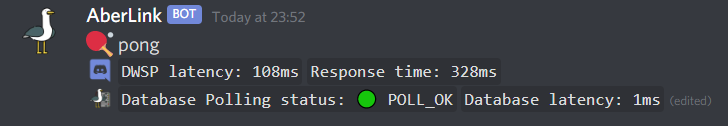
\includegraphics[width=1\linewidth]{Figures/discord-ping-command.png}
	\caption{Example of ping command in Discord}
	\label{fig:discord-command-ping}
\end{figure}

\subsection{How do I access a list of the commands in AberLink?}
The Discord.py library contains a useful function called \verb|DefaultHelpCommand()| that will generate an automatic list of commands available in your program by analysing each function that has the command decorator \verb|@commands.command()|. The list of commands is then accessible through Discord using the command prefix plus the keyword help which in this case would be !help. Below is an example of the current output from the help command at time of this screenshot.  

\begin{figure}[H]
	\centering
	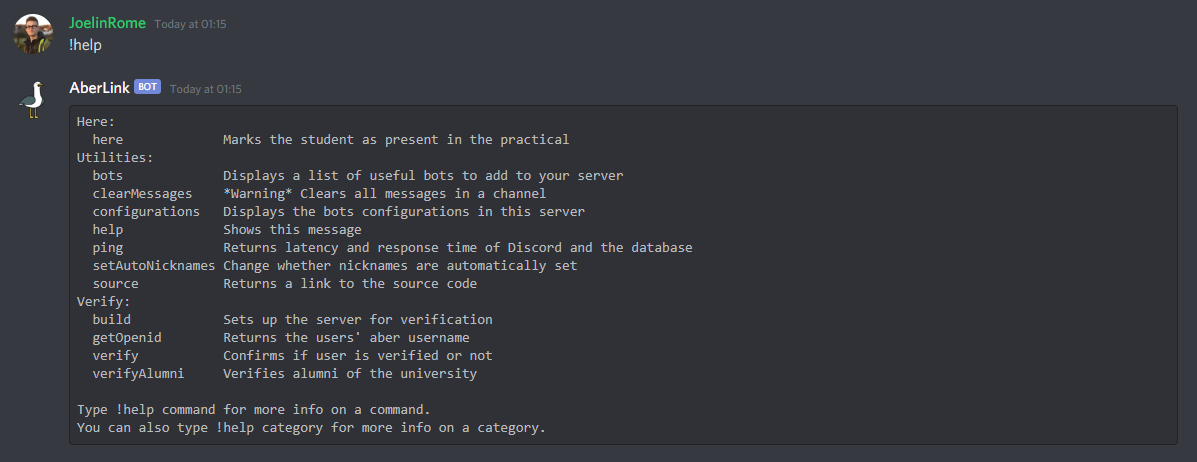
\includegraphics[width=1\linewidth]{Figures/discord-help.png}
	\caption{Example of Discord help command to display list of Discord commands for AberLink}
	\label{fig:discord-help}
\end{figure}

\subsection{Database}
The Discord bot uses the Python library psycopg2 \cite{psycopg2} to connect remotely to the PostgreSQL \cite{psql} database using a file located inside of the \verb|AberLinkDiscord/cogs| folder called \verb|db.py|.

\begin{figure}[H]
\begin{lstlisting}[language=Python]
CONN = 0

def connect():
"""
Connects or reconnects to database
"""
load_dotenv(find_dotenv())
DB_NAME = os.getenv('DATABASE_NAME')
DB_USER = os.getenv('USER')
DB_PASSWORD = os.getenv('PASSWORD')
DB_HOST = os.getenv('HOST')
DB_PORT = os.getenv('PORT')

try:
	global CONN
	CONN = psycopg2.connect(database=DB_NAME, user=DB_USER, password=DB_PASSWORD, host=DB_HOST, port=DB_PORT)
	print(f'Reconnected to PSQL database: {CONN}')
except psycopg2.OperationalError as err:
	print(f'Error connecting to database. Error: {err}')
	raise
\end{lstlisting}
\caption{Extract of the connection function to the PostgreSQL database from the AberLink Discord bot}
\label{fig:discord-database}
\end{figure}

As seen in the code extract above it uses the same functions as described in section \ref{sec3:discord-setup} for loading data from the \verb|.env|. Once it has loaded in the correct key value pairs it then attempts to connect to the database using the function \verb|connect()| and print the output to the command line. If this is not the case e.g. database is down then then the try except statement catches the error and prints it out to the command line. If the database connection is successful however the information about that connection is then stored in a global variable called \verb|CONN| which stands for connection.

To ensure that the connection will always be restored if there is a catastrophic failure a function was added that attempts to get a cursor on the database and if it fails then it calls the function above in figure \ref{fig:discord-database}. This function \verb|try_connection()| is called by any piece of code that relies on extracting information from the database to ensure that there will never be a database error.

\begin{figure}[H]
\begin{lstlisting}[language=Python]
def try_connection():
	"""
	Attempts to get a cursor from the database otherwise it restarts the database connection
	"""
	try:
		cur = CONN.cursor()
	except psycopg2.InterfaceError:
		PostgreSQL.connect()
\end{lstlisting}
\caption{Extract of the try connection function for connecting to the database from the Discord bot}
\label{fig:discord-database-try-connect}
\end{figure}

Once a connection is established with the database and connection issues are handled then SQL queries can be made on the database to get information. In Discord there are only really two functions that are required to read information on a student; a function to lookup a students Discord account using their Discord ID and a function to lookup a students Aber OpenID Connect information using their username. Both of these functions are relatively similar so only one has been included to illustrate how this works.

\begin{figure}[H]
\begin{lstlisting}[language=Python]
def get_discord_user(discord_id: int):
""" 
Returns a discord user if they exist or None
"""
PostgreSQL.try_connection()
cur = CONN.cursor()

cur.execute(f"SELECT * FROM login_discorduser WHERE id={discord_id}")
row = cur.fetchone()
if row is not None:
	return {"id": row[0], "last_login": row[1], "openidc_id": row[2]}
\end{lstlisting}
\caption{SQL function used to get information on a Discord user from the database in the Discord bot}
\label{fig:discord-database-sql-statement}
\end{figure}

As seen above a parameter of the Discord ID is passed to the function which then gets a database connection using the \verb|try_connect()| as previously described in the last section and executes an SQL statement on the database. The first record is then fetched from the database and is then returned as a JSON object to allow for it to be easily accessed. If there are no records that match then None is returned.

\subsection{Verification}
This command is used to verify users accounts. It begins by trying to find the verified role on the server, then using the function above in figure \ref{fig:discord-database-sql-statement} to get the users information. The function then checks that the user exists and then uses another SQL lookup to get information on the OpenID Connect \cite{OpenID} Aber account. Once these requests have been completed the user is given the role of \verb|verified| followed by the message "You are now verified with AberLink". If the feature discussed in section \ref{sec3:server-config} to allow automatic nicknames is enabled then the bot will also change the users nickname.

\begin{figure}[H]
\begin{lstlisting}[language=Python]
@commands.bot_has_permissions(manage_nicknames=True, manage_roles=True)
@commands.command(aliases=['v'])
async def verify(self, ctx: Context):
	"""
	Confirms if user is verified or not
	"""
	verified = await check_verify_role(ctx)
	db_discord_user = await check_discord_user(ctx)
	if verified is None or db_discord_user is None:
		return
	db_openid_user = PostgreSQL.get_openid_user(db_discord_user["openidc_id"])
	email = db_openid_user["username"]
	user = ctx.message.author
	await user.add_roles(verified, reason='Assigning user the verified role')
	await ctx.send("You are now verified with AberLink")

	if check_shelve_file(ctx.guild):
        await user.edit(nick=f'{user.name} [{email}]', reason="Changing users\'s nickname")
\end{lstlisting}
\caption{Discord command to verify students}
\label{fig:discord-verify-cmd}
\end{figure}

\subsection{Attendance}
Attendance is recorded using the Discord function \verb|here|. Once the command has been typed then the Discord bot will delete the message and open a DM or Direct Message with the user. It then sends a query to the database and if the user exists then a query is made to retrieve their aber account. After this is completed a request is made to the API endpoint along with the data object \verb|{'username': <aber_email>}| which updates student record. The response from this request is then evaluated and an appropriate response is sent via the DM channel that was opened earlier.

\begin{figure}[H]
\begin{lstlisting}[language=Python]
@commands.command(aliases=['h'])
async def here(self, ctx: Context):
	"""
	Marks the student as present in the practical
	"""
	await ctx.message.delete()
	dm_channel = await ctx.author.create_dm()
	discord_user = PostgreSQL.get_discord_user(ctx.author.id)
	url = 'https://integration.aber.ac.uk/joa38/submit.php'

	# Gets openid user from Discord id
	if discord_user is None:
		await dm_channel.send(f'You have not been verified yet. Please visit {WEBSITE} to get verified')
		return
	openid_user = PostgreSQL.get_openid_user(discord_user["openidc_id"])

	# getting request from API endpoint
	data = {'username': openid_user["username"]}
	api_response = requests.post(url, json=data).json()

	# If evaluates to true send user message with timestamp
	if eval(api_response["status_updated"].title()):
		current_time = datetime.now()
		current_time = current_time.strftime("%d/%m/%Y %H:%M:%S")
		await dm_channel.send(f'Your attendance in the server `{ctx.guild.name}` has been recorded for the module: `{api_response["module_code"]}` with timestamp: `{current_time}`')
	else:
		await dm_channel.send('Your attendance has not been recorded for this practical. If you believe this is incorrect please contact your module coordinator.')
\end{lstlisting}
\caption{Discord command to mark students attendance}
\label{fig:discord-here-cmd}
\end{figure}

\subsection{Error handling}
Discord.py includes a decorator called \verb|@Bot.event()| that goes inside of the AberLink.py file for dealing with bot events. This paired with a function called \verb|on_command_error()| deals with error messages. Below is an example of some of the if statements that deal with bot errors. The final else if command to check if the command is not found is extremely important as it tells the bot to ignore any commands that does not exist in the case where two Discord bots use the same command prefix but have different commands.

\begin{figure}[H]
\begin{lstlisting}[language=Python]
if isinstance(error, commands.errors.CheckFailure):
	await ctx.send(error)
elif isinstance(error, commands.errors.MissingRequiredArgument):
	await ctx.send('You are missing a required argument.')
elif isinstance(error, commands.errors.CommandNotFound):
	pass
\end{lstlisting}
\caption{Example of AberLink's on\_command\_error() checking statements}
\label{fig:discord-error-checking}
\end{figure}

\subsection{Server Configurations}\label{sec3:server-config}
AberLink contains a feature called autoSetNickname that will automatically assign nicknames to users when they join or verify on the server by appending their aber username to the end of their name. e.g. JoelinRome\#4893 becomes JoelinRome [joa38]. This was added to help lecturers easily identify which student is which and if the student is uncomfortable with this they can always manually change it back. 

Some lecturers might not enjoy this feature and prefer to turn it off so included is a micro database using the python module \cite{shelve} that creates a file stored in the same directory as the Python file. This basically creates a file that can be accessed at any time and acts as persistent storage. It contains key value pairs e.g. \verb|{server_id : true}| that store a boolean on whether the automatic naming feature is enabled or disabled. 

\section{Database}\label{sec3:database}
The Database implementation was relatively straight forward as Django \cite{Django} generates all of the required tables for the project to function once you define the models. I've included the model used to generate OpenID Connect \cite{OpenID} aber user model below. In this figure you can see that there are two classes; OpenIDCUserManager to create a new database object and OpenIDCUser to make the database model. 

The OpenIDCUserManager class has three main parameters; one to call itself, a user which is a JSON object and password which is defaulted to None as no password data is stored. The information from the user object is passed throughout the code and is used to decide if the user should have admin permissions. The user is then saved to the database.

The OpenIDCUser class contains a nested class called usertypes that is a list of all the possible choices for incoming usertypes from user authentication. Further down we can see that there is a set of definitions for the database model such as the id, username, name, etc. Note however that the usertype definition uses the choices class to define what role a user may have. As this model is the main model used to authenticate users on the website Django requires that the model contains a few special items including a password which I have set to None and the arrays at the bottom called USERNAME\_FIELD and REQUIRED\_FIELDS.

\begin{figure}[H]
\begin{lstlisting}[language=Python]
class OpenIDCUserManager(BaseUserManager):
    def create_user(self, user, password=None):
        new_user = self.model(
            username = user['OIDC_CLAIM_preferred_username'],
            name = user['OIDC_CLAIM_name'],
            email = user['OIDC_CLAIM_email'],
            usertype = user['OIDC_CLAIM_usertype']
        )
        if user['OIDC_CLAIM_usertype'] == "staff":
            new_user.is_admin = True
        new_user.save(using=self._db)
        return new_user

class OpenIDCUser(AbstractBaseUser):
    objects = OpenIDCUserManager()

    class usertypes(models.TextChoices):
        STAFF = 'staff'
        UNDERGRAD = 'undergrad'
        POSTGRAD = 'postgrad'
        OFFICE = 'office'
        CONTED = 'conted'
        SUMMER = 'summer'
        WEB = 'web'
        TEMPORARY = 'temporary'
        UNKNOWN = 'unknown'

    id = models.AutoField(auto_created=True, primary_key=True, serialize=False)
    username = models.CharField(max_length=40)
    name = models.CharField(max_length=300)
    email = models.CharField(max_length=30)
    usertype = models.CharField(max_length=50, choices=usertypes.choices)
    last_login = models.DateTimeField(null=True)
    password = None
    is_active = models.BooleanField(default=True)
    is_admin = models.BooleanField(default=False)

    USERNAME_FIELD = 'id'
    REQUIRED_FIELDS = ['username', 'name', 'email', 'usertype']
\end{lstlisting}
\caption{Django database model of OpenID Connect Aber users}
\label{fig:django-database-code}
\end{figure}

The tables generated for the database are pictured below and they do differ quite drastically from the tables discussed during the design section \ref{sec2:database} of this document. This is because I was not originally accounting for the tables that get automatically generated by Django \cite{Django} that are required for the application to run. Below the figure is information to explain what the Django generated tables mean.

\begin{figure}[H]
	\centering
	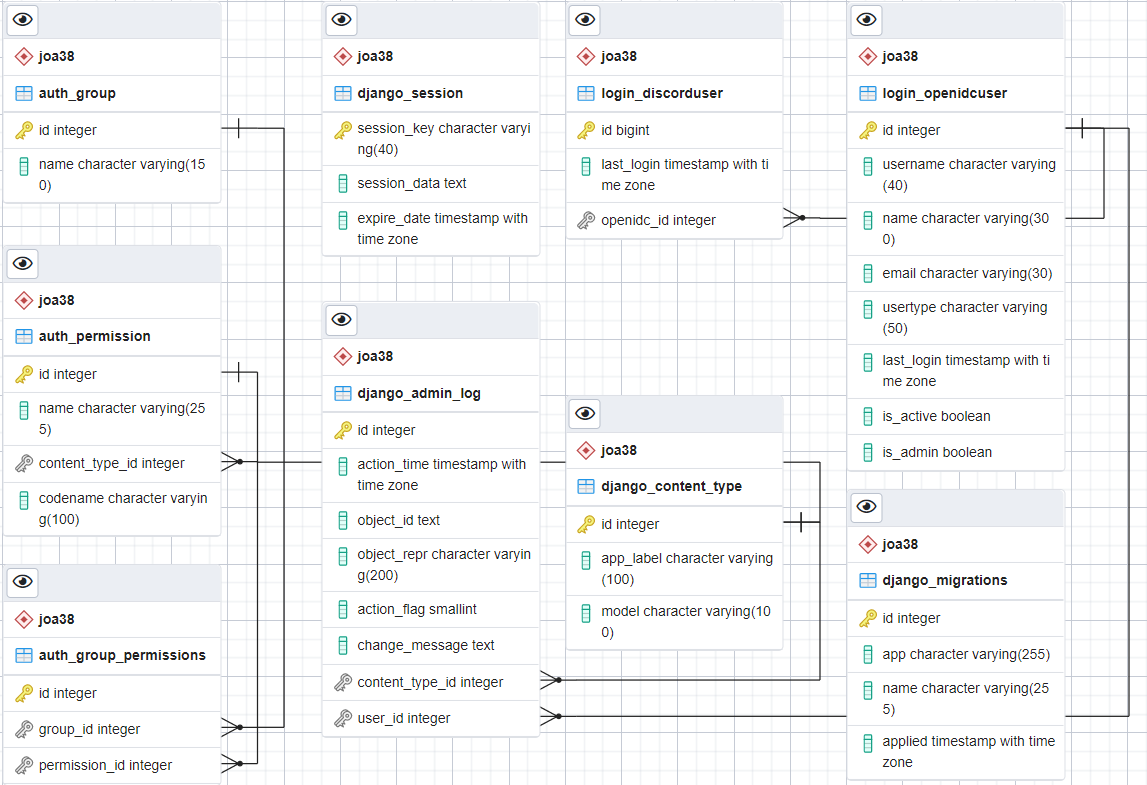
\includegraphics[width=1\linewidth]{Figures/er-diagram.png}
	\caption{Final Entity Relationship diagram for database}
	\label{fig:final-database}
\end{figure}

\begin{itemize}
	\item \textbf{User tables} - These two tables are the ones that have been discussed previously in this document for storing user data.
	\begin{itemize}
		\item \textbf{login\_openidcuser} - This table stores the OpenID Connect \cite{OpenID} information and is used as the authenticated user account.
		\item \textbf{login\_discorduser} - This table stores information on the discord user and contains a foreign key relationship with the table above.
	\end{itemize}
	\item \textbf{Django tables} - Tables generated by Django \cite{Django}
	\begin{itemize}
		\item \textbf{django\_migrations} - This table contains the history of the changes made to the database using Django. It acts as a way to revert to previous versions of the database in the case of 
		errors.
		\item \textbf{django\_session} - Stores sessions on the currently logged in users.
		\item \textbf{django\_content\_type} - Stores information on all available models in the database.
		\item \textbf{django\_admin\_log} - Stores history of logins for administrative users.
		\item \textbf{auth\_group \& auth\_group\_permissions \& auth\_permissions} - These tables are part of the backend for the authentication of users.
	\end{itemize}
\end{itemize}

Below are examples of the records that are stored in the database tables. 

\textbf{Note}: The column last\_login in the table \ref{tab:aber-table} contains the word datetime but should have a datetime object as seen in table \ref{tab:dis-table}. It has been removed so that the table fits nicely in this document.

\begin{table}[H]
	\centering
	\small
	\setlength\tabcolsep{2pt}
	\begin{tabular}{|c|c|c|c|c|c|c|c|}
		\hline
		\underline{id} & username & name & email & usertype & last\_login & is\_active & is\_admin \\
		\hline
		1 & joa38 & Joel Adams & joa38@aber.ac.uk & staff & datetime & t & t \\
		2 & jet39 & Jenny Thyer & jet39@aber.ac.uk & student & datetime & t & f \\
		3 & maw86 & Michael Antony West & maw86@aber.ac.uk & student & datetime & t & f \\
		\hline 
	\end{tabular}
	\caption{Aberystwyth user table example}
	\label{tab:aber-table}
\end{table}

\begin{table}[H]
	\centering
	\small
	\setlength\tabcolsep{2pt}
	\begin{tabular}{|c|c|c|}
		\hline
		\underline{id}                 & last\_login                   & openidc\_id* \\
		\hline
		727834884915331144 & 2021-02-18 16:43:47.067328+00 & 1           \\
		284352754321719296 & 2021-02-18 16:43:47.067328+00 & 1           \\
		246998944964542464 & 2021-02-04 11:14:40.057891+00 & 2           \\
		282248714955784192 & 2021-02-12 17:35:23.044226+00 & 3           \\
		\hline
	\end{tabular}
	\caption{Discord user table example}
	\label{tab:dis-table}
\end{table}

\section{Configuration and Setup}
After completion of this project there is a plan to setup this service permanently for the department so a folder was created called \verb|config| containing information on how to set up this project. This folder contains a \verb|README.md| file located in Appendix D that explains how and what is needed to be configured to get the system up and running properly. it also contains a bash script called \verb|setup.sh| that installs and the relevant dependencies and sets up the virtual environments for the projects. Also included are a few example configuration files for Apache2 \cite{apache2}, Django \cite{Django}, OpenID Connect authentication \cite{OpenID} and Discord.py \cite{discord.py}.

\section{Unforeseen Issues}\label{sec3:unforeseen}
An issue that was encountered was with creating the custom user model in Django that would have been used to model the database. The documentation and videos found online about implementing user models were rather cryptic and difficult to understand, however after much research a video explaining how to implement a good custom user model was found that resolved the issues. Once this was completed I realised that Django is not happy with modelling the primary key of a table using a char so switched over to using an int. This turned out to be a good idea as Aberystwyth University tends to recycle old emails so over the next 5 years there could be an issue where the database would try and create a new entry in the database with the same email.
\begin{figure}[H]
	\centering
	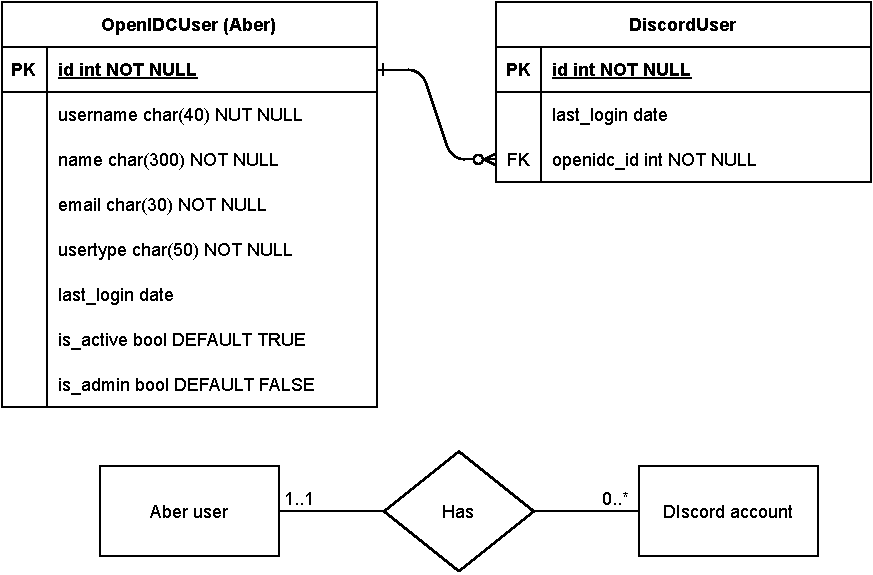
\includegraphics[width=0.8\linewidth]{Figures/database-er-1}
	\caption{Updated Entity relationship diagram for database}
	\label{fig:database-er-1}
\end{figure}

\section{Review}
\subsection{Review Against Planned Requirements}\label{sec3:pr}
Most of the planned requirements have not changed during implementation however some of the promised tasks have only been partially fulfilled. Please see Appendix \ref{tab:fr-test} for a table of the functional requirements specified in \ref{sec1:fr}. For more information on requirements that did not pass please see \ref{sec4:fr}.

In the final section of section \ref{sec1:obj} \textbf{Further potential work} I have decided against integrating DemoHelper into AberLink as this would greatly increase its complexity and make it much more difficult to maintain. Welsh language support has also not been implemented as I do not speak the language nor understand it well enough.

\subsection{Review Against Project Process}\label{sec3:pp}

Below is included a table describing the iterations and what was completed each one. These iterations were based on the list of objectives created in section \ref{sec1:obj} and span over the course of two months. For more detail please see the wordpress blog here \href{https://cs39440blog.wordpress.com/}{https://cs39440blog.wordpress.com/}.
\newpage
\begin{longtable}[H]{| c | c | p{9cm} |}
\hline
Iteration & Time taken (days) & What happened? \\
\hline
1 & 5 & Research into services required to run the project and basic setup of University container. Lots of meetings to discuss what data can be used/stored and began setup of API endpoint for attendance. \\
\hline
2 & 5 & Setup HTTPS on container, installed Django \cite{Django} and created basic website using it. Linked up Django to database and created basic Discord login system. \\
\hline
3 & 5 & Added OpenID Connect \cite{OpenID} to website for aber user login. Created basic models to link OpenID accounts to Discord accounts in PostgreSQL \cite{psql}. \\
\hline
4 & 7 & Created Admin pages and implemented proper database model for Discord and Aber users\\
\hline
5 & 5 & Created Discord bot skeleton and added support for it to connect to the database.\\
\hline
6 & 5 & Added attendance and verification to Discord bot. \\
\hline
7 & 5 & Added content to main webpage and option to delete a Discord account or all data. Added custom error message webpages for 400, 403, 404 and 500. \\
\hline
8 & 5 & Updated main user page so that it queries Discord API to get profile picture and username and update webpage with details. Added more features to Discord bot to interact with database.\\
\hline
9 & 5 & Created Configuration folder for installing the software along with bash script to install dependencies.\\
\hline
10 & 5 & Added Discord bot functionality to add configurations to a server and feature to automatically change Discord users nickname to append aber email.\\
\hline
11 & 16 & Working on LaTeX document for project report. \\
\hline
\caption{Project iterations and what occurred}
\label{tab:project-iterations}
\end{longtable}

Included is a graph of GitLab commits over time below to reflect the tables results as described above. 

\begin{figure}[H]
	\centering
	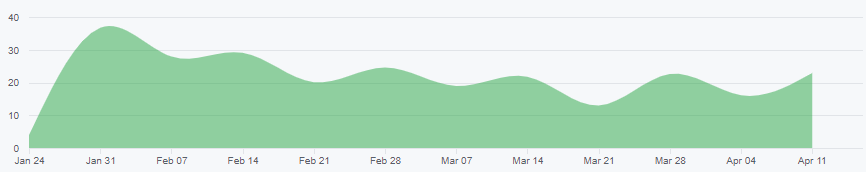
\includegraphics[width=1\linewidth]{Figures/gitlab-commit-graph.png}
	\caption{GitLab graph of commits over time}
	\label{fig:gitlab-graph}
\end{figure}